\chapter{Grafos dirigidos}

En este capítulo, nos centramos en dos clases de grafos dirigidos:
\begin{itemize}
\item \key{Grafos acíclicos}:
No hay ciclos en el grafo,
por lo que no hay camino desde ningún nodo hasta sí mismo\footnote{Los grafos acíclicos dirigidos a veces se denominan DAGs.}.
\item \key{Grafos sucesores}:
El grado de salida de cada nodo es 1,
por lo que cada nodo tiene un sucesor único.
\end{itemize}
Resulta que en ambos casos,
podemos diseñar algoritmos eficientes que se basan
en las propiedades especiales de los grafos.

\section{Ordenación topológica}

\index{ordenación topológica}
\index{ciclo}

Una \key{ordenación topológica} es una ordenación
de los nodos de un grafo dirigido
tal que si hay un camino desde el nodo $a$ hasta el nodo $b$,
entonces el nodo $a$ aparece antes que el nodo $b$ en la ordenación.
Por ejemplo, para el grafo
\begin{center}
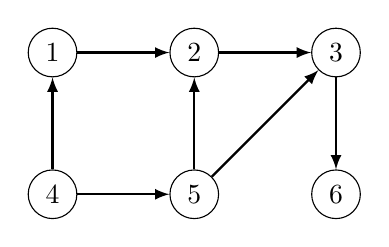
\begin{tikzpicture}[scale=0.9]
\node[draw, circle] (1) at (1,5) {$1$};
\node[draw, circle] (2) at (3,5) {$2$};
\node[draw, circle] (3) at (5,5) {$3$};
\node[draw, circle] (4) at (1,3) {$4$};
\node[draw, circle] (5) at (3,3) {$5$};
\node[draw, circle] (6) at (5,3) {$6$};

\path[draw,thick,->,>=latex] (1) -- (2);
\path[draw,thick,->,>=latex] (2) -- (3);
\path[draw,thick,->,>=latex] (4) -- (1);
\path[draw,thick,->,>=latex] (4) -- (5);
\path[draw,thick,->,>=latex] (5) -- (2);
\path[draw,thick,->,>=latex] (5) -- (3);
\path[draw,thick,->,>=latex] (3) -- (6);
\end{tikzpicture}
\end{center}
una ordenación topológica es
$[4,1,5,2,3,6]$:
\begin{center}
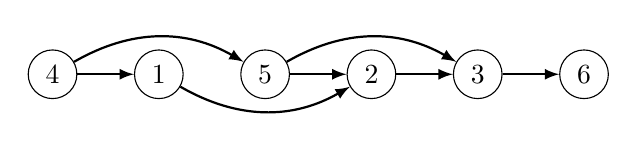
\begin{tikzpicture}[scale=0.9]
\node[draw, circle] (1) at (-6,0) {$1$};
\node[draw, circle] (2) at (-3,0) {$2$};
\node[draw, circle] (3) at (-1.5,0) {$3$};
\node[draw, circle] (4) at (-7.5,0) {$4$};
\node[draw, circle] (5) at (-4.5,0) {$5$};
\node[draw, circle] (6) at (-0,0) {$6$};

\path[draw,thick,->,>=latex] (1) edge [bend right=30] (2);
\path[draw,thick,->,>=latex] (2) -- (3);
\path[draw,thick,->,>=latex] (4) -- (1);
\path[draw,thick,->,>=latex] (4) edge [bend left=30] (5);
\path[draw,thick,->,>=latex] (5) -- (2);
\path[draw,thick,->,>=latex] (5) edge [bend left=30]  (3);
\path[draw,thick,->,>=latex] (3) -- (6);
\end{tikzpicture}
\end{center}

Un grafo acíclico siempre tiene una ordenación topológica.
Sin embargo, si el grafo contiene un ciclo,
no es posible formar una ordenación topológica,
porque ningún nodo del ciclo puede aparecer
antes que los demás nodos del ciclo en la ordenación.
Resulta que la búsqueda en profundidad se puede utilizar
para comprobar si un grafo dirigido contiene un ciclo
y, si no contiene un ciclo, para construir una ordenación topológica.

\subsubsection{Algoritmo}

La idea es recorrer los nodos del grafo
y siempre comenzar una búsqueda en profundidad en el nodo actual
si aún no se ha procesado.
Durante las búsquedas, los nodos tienen tres estados posibles:

\begin{itemize}
\item estado 0: el nodo no se ha procesado (blanco)
\item estado 1: el nodo está en proceso (gris claro)
\item estado 2: el nodo se ha procesado (gris oscuro)
\end{itemize}

Inicialmente, el estado de cada nodo es 0.
Cuando una búsqueda llega a un nodo por primera vez,
su estado pasa a ser 1.
Finalmente, después de que todos los sucesores del nodo hayan
sido procesados, su estado pasa a ser 2.

Si el grafo contiene un ciclo, nos daremos cuenta de esto
durante la búsqueda, porque tarde o temprano
llegaremos a un nodo cuyo estado es 1.
En este caso, no es posible construir una ordenación topológica.

Si el grafo no contiene un ciclo, podemos construir
una ordenación topológica agregando cada nodo a una lista cuando el estado del nodo pasa a ser 2.
Esta lista en orden inverso es una ordenación topológica.

\subsubsection{Ejemplo 1}

En el grafo de ejemplo, la búsqueda primero avanza
desde el nodo 1 hasta el nodo 6:

\begin{center}
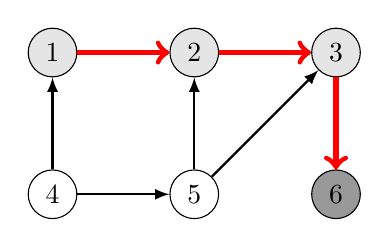
\begin{tikzpicture}[scale=0.9]
\node[draw, circle,fill=gray!20] (1) at (1,5) {$1$};
\node[draw, circle,fill=gray!20] (2) at (3,5) {$2$};
\node[draw, circle,fill=gray!20] (3) at (5,5) {$3$};
\node[draw, circle] (4) at (1,3) {$4$};
\node[draw, circle] (5) at (3,3) {$5$};
\node[draw, circle,fill=gray!80] (6) at (5,3) {$6$};

\path[draw,thick,->,>=latex] (4) -- (1);
\path[draw,thick,->,>=latex] (4) -- (5);
\path[draw,thick,->,>=latex] (5) -- (2);
\path[draw,thick,->,>=latex] (5) -- (3);
%\path[draw,thick,->,>=latex] (3) -- (6);

\path[draw=red,thick,->,line width=2pt] (1) -- (2);
\path[draw=red,thick,->,line width=2pt] (2) -- (3);
\path[draw=red,thick,->,line width=2pt] (3) -- (6);
\end{tikzpicture}
\end{center}

Ahora el nodo 6 se ha procesado, por lo que se agrega a la lista.
Después de esto, también los nodos 3, 2 y 1 se agregan a la lista:

\begin{center}
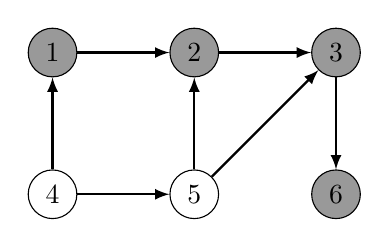
\begin{tikzpicture}[scale=0.9]
\node[draw, circle,fill=gray!80] (1) at (1,5) {$1$};
\node[draw, circle,fill=gray!80] (2) at (3,5) {$2$};
\node[draw, circle,fill=gray!80] (3) at (5,5) {$3$};
\node[draw, circle] (4) at (1,3) {$4$};
\node[draw, circle] (5) at (3,3) {$5$};
\node[draw, circle,fill=gray!80] (6) at (5,3) {$6$};
\path[draw,thick,->,>=latex] (1) -- (2);
\path[draw,thick,->,>=latex] (2) -- (3);
\path[draw,thick,->,>=latex] (4) -- (1);
\path[draw,thick,->,>=latex] (4) -- (5);
\path[draw,thick,->,>=latex] (5) -- (2);
\path[draw,thick,->,>=latex] (5) -- (3);
\path[draw,thick,->,>=latex] (3) -- (6);
\end{tikzpicture}
\end{center}

En este punto, la lista es $[6,3,2,1]$.
La próxima búsqueda comienza en el nodo 4:

\begin{center}
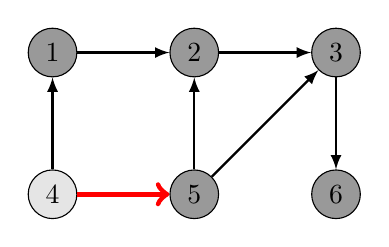
\begin{tikzpicture}[scale=0.9]
\node[draw, circle,fill=gray!80] (1) at (1,5) {$1$};
\node[draw, circle,fill=gray!80] (2) at (3,5) {$2$};
\node[draw, circle,fill=gray!80] (3) at (5,5) {$3$};
\node[draw, circle,fill=gray!20] (4) at (1,3) {$4$};
\node[draw, circle,fill=gray!80] (5) at (3,3) {$5$};
\node[draw, circle,fill=gray!80] (6) at (5,3) {$6$};

\path[draw,thick,->,>=latex] (1) -- (2);
\path[draw,thick,->,>=latex] (2) -- (3);
\path[draw,thick,->,>=latex] (4) -- (1);
%\path[draw,thick,->,>=latex] (4) -- (5);
\path[draw,thick,->,>=latex] (5) -- (2);
\path[draw,thick,->,>=latex] (5) -- (3);
\path[draw,thick,->,>=latex] (3) -- (6);

\path[draw=red,thick,->,line width=2pt] (4) -- (5);
\end{tikzpicture}
\end{center}

Por lo tanto, la lista final es $[6,3,2,1,5,4]$.
Hemos procesado todos los nodos, por lo que se ha encontrado
una ordenación topológica.
La ordenación topológica es la lista inversa
$[4,5,1,2,3,6]$:

\begin{center}
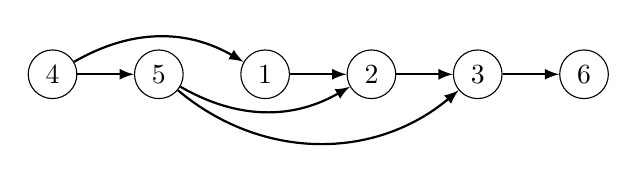
\begin{tikzpicture}[scale=0.9]
\node[draw, circle] (1) at (3,0) {$1$};
\node[draw, circle] (2) at (4.5,0) {$2$};
\node[draw, circle] (3) at (6,0) {$3$};
\node[draw, circle] (4) at (0,0) {$4$};
\node[draw, circle] (5) at (1.5,0) {$5$};
\node[draw, circle] (6) at (7.5,0) {$6$};

\path[draw,thick,->,>=latex] (1) -- (2);
\path[draw,thick,->,>=latex] (2) -- (3);
\path[draw,thick,->,>=latex] (4) edge [bend left=30] (1);
\path[draw,thick,->,>=latex] (4) -- (5);
\path[draw,thick,->,>=latex] (5) edge [bend right=30] (2);
\path[draw,thick,->,>=latex] (5) edge [bend right=40] (3);
\path[draw,thick,->,>=latex] (3) -- (6);
\end{tikzpicture}
\end{center}

Tenga en cuenta que una ordenación topológica no es única,
y puede haber varias ordenaciones topológicas para un gráfico.

\subsubsection{Ejemplo 2}

Consideremos ahora un gráfico para el cual no podemos
construir una ordenación topológica,
porque el gráfico contiene un ciclo:

\begin{center}
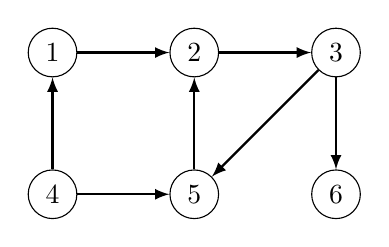
\begin{tikzpicture}[scale=0.9]
\node[draw, circle] (1) at (1,5) {$1$};
\node[draw, circle] (2) at (3,5) {$2$};
\node[draw, circle] (3) at (5,5) {$3$};
\node[draw, circle] (4) at (1,3) {$4$};
\node[draw, circle] (5) at (3,3) {$5$};
\node[draw, circle] (6) at (5,3) {$6$};

\path[draw,thick,->,>=latex] (1) -- (2);
\path[draw,thick,->,>=latex] (2) -- (3);
\path[draw,thick,->,>=latex] (4) -- (1);
\path[draw,thick,->,>=latex] (4) -- (5);
\path[draw,thick,->,>=latex] (5) -- (2);
\path[draw,thick,->,>=latex] (3) -- (5);
\path[draw,thick,->,>=latex] (3) -- (6);
\end{tikzpicture}
\end{center}
La búsqueda procede de la siguiente manera:
\begin{center}
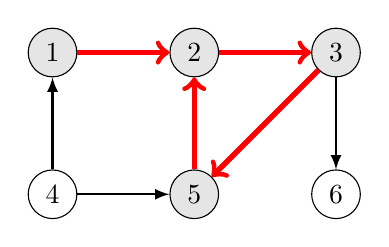
\begin{tikzpicture}[scale=0.9]
\node[draw, circle,fill=gray!20] (1) at (1,5) {$1$};
\node[draw, circle,fill=gray!20] (2) at (3,5) {$2$};
\node[draw, circle,fill=gray!20] (3) at (5,5) {$3$};
\node[draw, circle] (4) at (1,3) {$4$};
\node[draw, circle,fill=gray!20] (5) at (3,3) {$5$};
\node[draw, circle] (6) at (5,3) {$6$};

\path[draw,thick,->,>=latex] (4) -- (1);
\path[draw,thick,->,>=latex] (4) -- (5);
\path[draw,thick,->,>=latex] (3) -- (6);

\path[draw=red,thick,->,line width=2pt] (1) -- (2);
\path[draw=red,thick,->,line width=2pt] (2) -- (3);
\path[draw=red,thick,->,line width=2pt] (3) -- (5);
\path[draw=red,thick,->,line width=2pt] (5) -- (2);
\end{tikzpicture}
\end{center}
La búsqueda llega al nodo 2 cuyo estado es 1,
lo que significa que el gráfico contiene un ciclo.
En este ejemplo, hay un ciclo
$2 \rightarrow 3 \rightarrow 5 \rightarrow 2$.

\section{Programación dinámica}

Si un gráfico dirigido es acíclico,
la programación dinámica se puede aplicar a él.
Por ejemplo, podemos resolver eficientemente los siguientes
problemas relacionados con las rutas desde un nodo de inicio
hasta un nodo final:

\begin{itemize}
\item ¿Cuántas rutas diferentes hay?
\item ¿Cuál es la ruta más corta/más larga?
\item ¿Cuál es el número mínimo/máximo de aristas en una ruta?
\item ¿Qué nodos aparecen ciertamente en cualquier ruta?
\end{itemize}

\subsubsection{Contando el número de rutas}

Como ejemplo, calculemos el número de rutas
desde el nodo 1 al nodo 6 en el siguiente gráfico:

\begin{center}
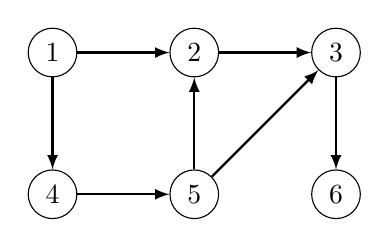
\begin{tikzpicture}[scale=0.9]
\node[draw, circle] (1) at (1,5) {$1$};
\node[draw, circle] (2) at (3,5) {$2$};
\node[draw, circle] (3) at (5,5) {$3$};
\node[draw, circle] (4) at (1,3) {$4$};
\node[draw, circle] (5) at (3,3) {$5$};
\node[draw, circle] (6) at (5,3) {$6$};
\path[draw,thick,->,>=latex] (1) -- (2);
\path[draw,thick,->,>=latex] (2) -- (3);
\path[draw,thick,->,>=latex] (1) -- (4);
\path[draw,thick,->,>=latex] (4) -- (5);
\path[draw,thick,->,>=latex] (5) -- (2);
\path[draw,thick,->,>=latex] (5) -- (3);
\path[draw,thick,->,>=latex] (3) -- (6);
\end{tikzpicture}
\end{center}
Hay un total de tres rutas de este tipo:
\begin{itemize}
\item $1 \rightarrow 2 \rightarrow 3 \rightarrow 6$
\item $1 \rightarrow 4 \rightarrow 5 \rightarrow 2 \rightarrow 3 \rightarrow 6$
\item $1 \rightarrow 4 \rightarrow 5 \rightarrow 3 \rightarrow 6$
\end{itemize}

Sea $\texttt{paths}(x)$ el número de rutas desde
el nodo 1 al nodo $x$.
Como caso base, $\texttt{paths}(1)=1$.
Entonces, para calcular otros valores de $\texttt{paths}(x)$,
podemos usar la recursión
\[\texttt{paths}(x) = \texttt{paths}(a_1)+\texttt{paths}(a_2)+\cdots+\texttt{paths}(a_k)\]
donde $a_1,a_2,\ldots,a_k$ son los nodos desde los que hay
una arista a $x$.
Dado que el gráfico es acíclico, los valores de $\texttt{paths}(x)$
se pueden calcular en el orden de una clasificación topológica.
Una clasificación topológica para el gráfico anterior es la siguiente:
\begin{center}
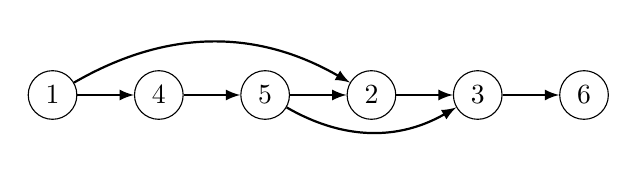
\begin{tikzpicture}[scale=0.9]
\node[draw, circle] (1) at (0,0) {$1$};
\node[draw, circle] (2) at (4.5,0) {$2$};
\node[draw, circle] (3) at (6,0) {$3$};
\node[draw, circle] (4) at (1.5,0) {$4$};
\node[draw, circle] (5) at (3,0) {$5$};
\node[draw, circle] (6) at (7.5,0) {$6$};

\path[draw,thick,->,>=latex] (1) edge [bend left=30] (2);
\path[draw,thick,->,>=latex] (2) -- (3);
\path[draw,thick,->,>=latex] (1) -- (4);
\path[draw,thick,->,>=latex] (4) -- (5);
\path[draw,thick,->,>=latex] (5) -- (2);
\path[draw,thick,->,>=latex] (5) edge [bend right=30] (3);
\path[draw,thick,->,>=latex] (3) -- (6);
\end{tikzpicture}
\end{center}
Por lo tanto, los números de rutas son los siguientes:
\begin{center}
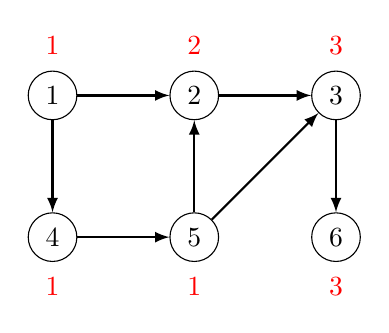
\begin{tikzpicture}[scale=0.9]
\node[draw, circle] (1) at (1,5) {$1$};
\node[draw, circle] (2) at (3,5) {$2$};
\node[draw, circle] (3) at (5,5) {$3$};
\node[draw, circle] (4) at (1,3) {$4$};
\node[draw, circle] (5) at (3,3) {$5$};
\node[draw, circle] (6) at (5,3) {$6$};

\path[draw,thick,->,>=latex] (1) -- (2);
\path[draw,thick,->,>=latex] (2) -- (3);
\path[draw,thick,->,>=latex] (1) -- (4);
\path[draw,thick,->,>=latex] (4) -- (5);
\path[draw,thick,->,>=latex] (5) -- (2);
\path[draw,thick,->,>=latex] (5) -- (3);
\path[draw,thick,->,>=latex] (3) -- (6);

\node[color=red] at (1,2.3) {$1$};
\node[color=red] at (3,2.3) {$1$};
\node[color=red] at (5,2.3) {$3$};
\node[color=red] at (1,5.7) {$1$};
\node[color=red] at (3,5.7) {$2$};
\node[color=red] at (5,5.7) {$3$};
\end{tikzpicture}
\end{center}

Por ejemplo, para calcular el valor de $\texttt{paths}(3)$,
podemos usar la fórmula $\texttt{paths}(2)+\texttt{paths}(5)$,
porque hay aristas desde los nodos 2 y 5
al nodo 3.
Dado que $\texttt{paths}(2)=2$ y $\texttt{paths}(5)=1$, concluimos que $\texttt{paths}(3)=3$.

\subsubsection{Extensión del algoritmo de Dijkstra}

\index{Algoritmo de Dijkstra}

Un subproducto del algoritmo de Dijkstra es un gráfico dirigido y acíclico
que indica para cada nodo del gráfico original
las formas posibles de alcanzar el nodo utilizando una ruta más corta
desde el nodo de inicio.
La programación dinámica se puede aplicar a ese gráfico.
Por ejemplo, en el gráfico
\begin{center}
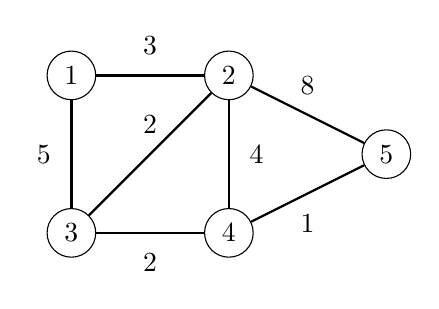
\begin{tikzpicture}
\node[draw, circle] (1) at (0,0) {$1$};
\node[draw, circle] (2) at (2,0) {$2$};
\node[draw, circle] (3) at (0,-2) {$3$};
\node[draw, circle] (4) at (2,-2) {$4$};
\node[draw, circle] (5) at (4,-1) {$5$};

\path[draw,thick,-] (1) -- node[font=\small,label=above:3] {} (2);
\path[draw,thick,-] (1) -- node[font=\small,label=left:5] {} (3);
\path[draw,thick,-] (2) -- node[font=\small,label=right:4] {} (4);
\path[draw,thick,-] (2) -- node[font=\small,label=above:8] {} (5);
\path[draw,thick,-] (3) -- node[font=\small,label=below:2] {} (4);
\path[draw,thick,-] (4) -- node[font=\small,label=below:1] {} (5);
\path[draw,thick,-] (2) -- node[font=\small,label=above:2] {} (3);
\end{tikzpicture}
\end{center}
las rutas más cortas desde el nodo 1 pueden usar las siguientes aristas:
\begin{center}
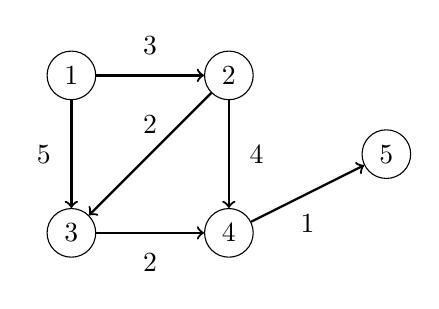
\begin{tikzpicture}
\node[draw, circle] (1) at (0,0) {$1$};
\node[draw, circle] (2) at (2,0) {$2$};
\node[draw, circle] (3) at (0,-2) {$3$};
\node[draw, circle] (4) at (2,-2) {$4$};
\node[draw, circle] (5) at (4,-1) {$5$};

\path[draw,thick,->] (1) -- node[font=\small,label=above:3] {} (2);
\path[draw,thick,->] (1) -- node[font=\small,label=left:5] {} (3);
\path[draw,thick,->] (2) -- node[font=\small,label=right:4] {} (4);
\path[draw,thick,->] (3) -- node[font=\small,label=below:2] {} (4);
\path[draw,thick,->] (4) -- node[font=\small,label=below:1] {} (5);
\path[draw,thick,->] (2) -- node[font=\small,label=above:2] {} (3);
\end{tikzpicture}
\end{center}
Ahora podemos, por ejemplo, calcular el número de
caminos más cortos desde el nodo 1 hasta el nodo 5
utilizando programación dinámica:
\begin{center}
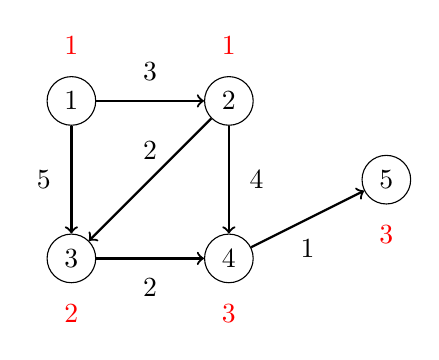
\begin{tikzpicture}
\node[draw, circle] (1) at (0,0) {$1$};
\node[draw, circle] (2) at (2,0) {$2$};
\node[draw, circle] (3) at (0,-2) {$3$};
\node[draw, circle] (4) at (2,-2) {$4$};
\node[draw, circle] (5) at (4,-1) {$5$};

\path[draw,thick,->] (1) -- node[font=\small,label=above:3] {} (2);
\path[draw,thick,->] (1) -- node[font=\small,label=left:5] {} (3);
\path[draw,thick,->] (2) -- node[font=\small,label=right:4] {} (4);
\path[draw,thick,->] (3) -- node[font=\small,label=below:2] {} (4);
\path[draw,thick,->] (4) -- node[font=\small,label=below:1] {} (5);
\path[draw,thick,->] (2) -- node[font=\small,label=above:2] {} (3);

\node[color=red] at (0,0.7) {$1$};
\node[color=red] at (2,0.7) {$1$};
\node[color=red] at (0,-2.7) {$2$};
\node[color=red] at (2,-2.7) {$3$};
\node[color=red] at (4,-1.7) {$3$};
\end{tikzpicture}
\end{center}

\subsubsection{Representando problemas como grafos}

En realidad, cualquier problema de programación dinámica
puede representarse como un grafo dirigido y acíclico.
En tal grafo, cada nodo corresponde a un estado de programación dinámica
y las aristas indican cómo los estados dependen unos de otros.

Como ejemplo, considere el problema
de formar una suma de dinero $n$
utilizando monedas
$\{c_1,c_2,\ldots,c_k\}$.
En este problema, podemos construir un grafo donde
cada nodo corresponde a una suma de dinero,
y las aristas muestran cómo se pueden elegir las monedas.
Por ejemplo, para las monedas $\{1,3,4\}$ y $n=6$,
el grafo es el siguiente:
\begin{center}
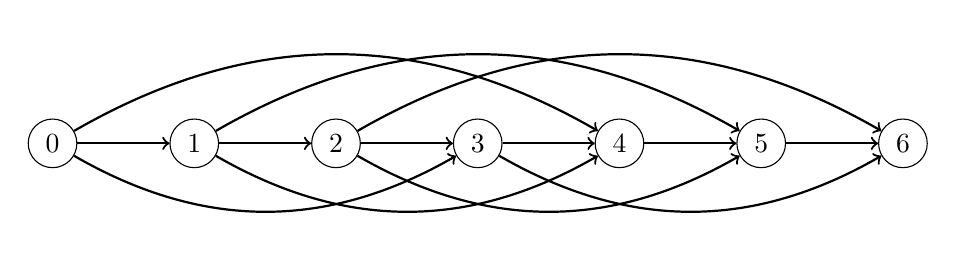
\begin{tikzpicture}[scale=0.9]
\node[draw, circle] (0) at (0,0) {$0$};
\node[draw, circle] (1) at (2,0) {$1$};
\node[draw, circle] (2) at (4,0) {$2$};
\node[draw, circle] (3) at (6,0) {$3$};
\node[draw, circle] (4) at (8,0) {$4$};
\node[draw, circle] (5) at (10,0) {$5$};
\node[draw, circle] (6) at (12,0) {$6$};

\path[draw,thick,->] (0) -- (1);
\path[draw,thick,->] (1) -- (2);
\path[draw,thick,->] (2) -- (3);
\path[draw,thick,->] (3) -- (4);
\path[draw,thick,->] (4) -- (5);
\path[draw,thick,->] (5) -- (6);

\path[draw,thick,->] (0) edge [bend right=30] (3);
\path[draw,thick,->] (1) edge [bend right=30] (4);
\path[draw,thick,->] (2) edge [bend right=30] (5);
\path[draw,thick,->] (3) edge [bend right=30] (6);

\path[draw,thick,->] (0) edge [bend left=30] (4);
\path[draw,thick,->] (1) edge [bend left=30] (5);
\path[draw,thick,->] (2) edge [bend left=30] (6);
\end{tikzpicture}
\end{center}

Usando esta representación,
el camino más corto desde el nodo 0 hasta el nodo $n$
corresponde a una solución con el número mínimo de monedas,
y el número total de caminos desde el nodo 0 hasta el nodo $n$
es igual al número total de soluciones.

\section{Caminos sucesores}

\index{grafo sucesor}
\index{grafo funcional}

Para el resto del capítulo,
nos centraremos en los \key{grafos sucesores}.
En esos grafos,
el grado de salida de cada nodo es 1, es decir,
exactamente una arista comienza en cada nodo.
Un grafo sucesor consiste en uno o más
componentes, cada uno de los cuales contiene
un ciclo y algunos caminos que conducen a él.

Los grafos sucesores a veces se llaman
\key{grafos funcionales}.
La razón de esto es que cualquier grafo sucesor
corresponde a una función que define
las aristas del grafo.
El parámetro de la función es un nodo del grafo,
y la función da el sucesor de ese nodo.

Por ejemplo, la función
\begin{center}
\begin{tabular}{r|rrrrrrrrr}
$x$ & 1 & 2 & 3 & 4 & 5 & 6 & 7 & 8 & 9 \\
\hline
$\texttt{succ}(x)$ & 3 & 5 & 7 & 6 & 2 & 2 & 1 & 6 & 3 \\
\end{tabular}
\end{center}
define el siguiente grafo:
\begin{center}
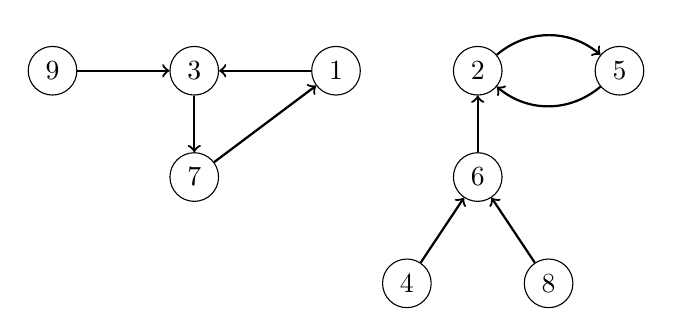
\begin{tikzpicture}[scale=0.9]
\node[draw, circle] (1) at (0,0) {$1$};
\node[draw, circle] (2) at (2,0) {$2$};
\node[draw, circle] (3) at (-2,0) {$3$};
\node[draw, circle] (4) at (1,-3) {$4$};
\node[draw, circle] (5) at (4,0) {$5$};
\node[draw, circle] (6) at (2,-1.5) {$6$};
\node[draw, circle] (7) at (-2,-1.5) {$7$};
\node[draw, circle] (8) at (3,-3) {$8$};
\node[draw, circle] (9) at (-4,0) {$9$};

\path[draw,thick,->] (1) -- (3);
\path[draw,thick,->] (2)  edge [bend left=40] (5);
\path[draw,thick,->] (3) -- (7);
\path[draw,thick,->] (4) -- (6);
\path[draw,thick,->] (5)  edge [bend left=40] (2);
\path[draw,thick,->] (6) -- (2);
\path[draw,thick,->] (7) -- (1);
\path[draw,thick,->] (8) -- (6);
\path[draw,thick,->] (9) -- (3);
\end{tikzpicture}
\end{center}

Dado que cada nodo de un grafo sucesor tiene un
sucesor único, también podemos definir una función $\texttt{succ}(x,k)$
que da el nodo al que llegaremos si
comenzamos en el nodo $x$ y caminamos $k$ pasos hacia adelante.
Por ejemplo, en el grafo anterior $\texttt{succ}(4,6)=2$,
porque llegaremos al nodo 2 caminando 6 pasos desde el nodo 4:


\begin{center}
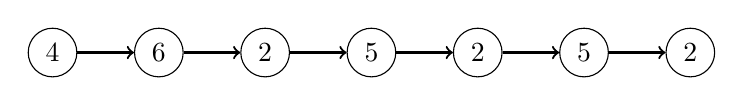
\begin{tikzpicture}[scale=0.9]
\node[draw, circle] (1) at (0,0) {$4$};
\node[draw, circle] (2) at (1.5,0) {$6$};
\node[draw, circle] (3) at (3,0) {$2$};
\node[draw, circle] (4) at (4.5,0) {$5$};
\node[draw, circle] (5) at (6,0) {$2$};
\node[draw, circle] (6) at (7.5,0) {$5$};
\node[draw, circle] (7) at (9,0) {$2$};

\path[draw,thick,->] (1) -- (2);
\path[draw,thick,->] (2) -- (3);
\path[draw,thick,->] (3) -- (4);
\path[draw,thick,->] (4) -- (5);
\path[draw,thick,->] (5) -- (6);
\path[draw,thick,->] (6) -- (7);
\end{tikzpicture}
\end{center}

Una forma sencilla de calcular un valor de $\texttt{succ}(x,k)$
es comenzar en el nodo $x$ y caminar $k$ pasos hacia adelante, lo que lleva $O(k)$ tiempo.
Sin embargo, utilizando el preprocesamiento, cualquier valor de $\texttt{succ}(x,k)$
se puede calcular en solo $O(\log k)$ tiempo.

La idea es precalcular todos los valores de $\texttt{succ}(x,k)$ donde
$k$ es una potencia de dos y como máximo $u$, donde $u$ es
el número máximo de pasos que alguna vez caminaremos.
Esto se puede hacer de manera eficiente, porque
podemos usar la siguiente recursión:

\begin{equation*}
    \texttt{succ}(x,k) = \begin{cases}
               \texttt{succ}(x)              & k = 1\\
               \texttt{succ}(\texttt{succ}(x,k/2),k/2)   & k > 1\\
           \end{cases}
\end{equation*}

Precalcular los valores lleva $O(n \log u)$ tiempo,
porque se calculan $O(\log u)$ valores para cada nodo.
En el gráfico anterior, los primeros valores son los siguientes:

\begin{center}
\begin{tabular}{r|rrrrrrrrr}
$x$ & 1 & 2 & 3 & 4 & 5 & 6 & 7 & 8 & 9 \\
\hline
$\texttt{succ}(x,1)$ & 3 & 5 & 7 & 6 & 2 & 2 & 1 & 6 & 3 \\
$\texttt{succ}(x,2)$ & 7 & 2 & 1 & 2 & 5 & 5 & 3 & 2 & 7 \\
$\texttt{succ}(x,4)$ & 3 & 2 & 7 & 2 & 5 & 5 & 1 & 2 & 3 \\
$\texttt{succ}(x,8)$ & 7 & 2 & 1 & 2 & 5 & 5 & 3 & 2 & 7 \\
$\cdots$ \\
\end{tabular}
\end{center}

Después de esto, cualquier valor de $\texttt{succ}(x,k)$ se puede calcular
presentando el número de pasos $k$ como una suma de potencias de dos.
Por ejemplo, si queremos calcular el valor de $\texttt{succ}(x,11)$,
primero formamos la representación $11=8+2+1$.
Usando eso,
\[\texttt{succ}(x,11)=\texttt{succ}(\texttt{succ}(\texttt{succ}(x,8),2),1).\]
Por ejemplo, en el gráfico anterior
\[\texttt{succ}(4,11)=\texttt{succ}(\texttt{succ}(\texttt{succ}(4,8),2),1)=5.\]

Tal representación siempre consiste en
$O(\log k)$ partes, por lo que calcular un valor de $\texttt{succ}(x,k)$
lleva $O(\log k)$ tiempo.

\section{Detección de ciclos}

\index{ciclo}
\index{detección de ciclos}

Considere un gráfico sucesor que solo contiene
una ruta que termina en un ciclo.
Podemos hacer las siguientes preguntas:
si comenzamos nuestra caminata en el nodo de inicio,
¿cuál es el primer nodo en el ciclo?
¿y cuántos nodos contiene el ciclo?

Por ejemplo, en el gráfico

\begin{center}
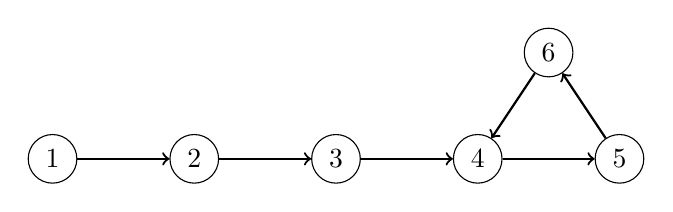
\begin{tikzpicture}[scale=0.9]
\node[draw, circle] (5) at (0,0) {$5$};
\node[draw, circle] (4) at (-2,0) {$4$};
\node[draw, circle] (6) at (-1,1.5) {$6$};
\node[draw, circle] (3) at (-4,0) {$3$};
\node[draw, circle] (2) at (-6,0) {$2$};
\node[draw, circle] (1) at (-8,0) {$1$};

\path[draw,thick,->] (1) -- (2);
\path[draw,thick,->] (2) -- (3);
\path[draw,thick,->] (3) -- (4);
\path[draw,thick,->] (4) -- (5);
\path[draw,thick,->] (5) -- (6);
\path[draw,thick,->] (6) -- (4);
\end{tikzpicture}
\end{center}
comenzamos nuestra caminata en el nodo 1,
el primer nodo que pertenece al ciclo es el nodo 4, y el ciclo consiste
en tres nodos (4, 5 y 6).

Una forma sencilla de detectar el ciclo es caminar en el
gráfico y hacer un seguimiento de
todos los nodos que se han visitado. Una vez que un nodo se visita
por segunda vez, podemos concluir
que el nodo es el primer nodo en el ciclo.
Este método funciona en $O(n)$ tiempo y también usa
$O(n)$ memoria.

Sin embargo, existen mejores algoritmos para la detección de ciclos.
La complejidad temporal de tales algoritmos sigue siendo $O(n)$,
pero solo usan $O(1)$ memoria.
Esta es una mejora importante si $n$ es grande.
A continuación, discutiremos el algoritmo de Floyd que
alcanza estas propiedades.

\subsubsection{Algoritmo de Floyd}

\index{algoritmo de Floyd}

\key{Algoritmo de Floyd}\footnote{La idea del algoritmo se menciona en \cite{knu982}
y se atribuye a R. W. Floyd; sin embargo, no se sabe si Floyd realmente
descubrió el algoritmo.} camina hacia adelante
en el gráfico utilizando dos punteros $a$ y $b$.
Ambos punteros comienzan en un nodo $x$ que
es el nodo de inicio del gráfico.
Luego, en cada turno, el puntero $a$ camina
un paso adelante y el puntero $b$
camina dos pasos adelante.
El proceso continúa hasta
que los punteros se encuentran entre sí:
\begin{lstlisting}
a = succ(x);
b = succ(succ(x));
while (a != b) {
    a = succ(a);
    b = succ(succ(b));
}
\end{lstlisting}


En este punto, el puntero $a$ ha caminado $k$ pasos
y el puntero $b$ ha caminado $2k$ pasos,
por lo que la longitud del ciclo divide $k$.
Por lo tanto, el primer nodo que pertenece al ciclo
se puede encontrar moviendo el puntero $a$ al nodo $x$
y avanzando los punteros
paso a paso hasta que se encuentren de nuevo.
\begin{lstlisting}
a = x;
while (a != b) {
    a = succ(a);
    b = succ(b);
}
first = a;
\end{lstlisting}

Después de esto, la longitud del ciclo
se puede calcular de la siguiente manera:
\begin{lstlisting}
b = succ(a);
length = 1;
while (a != b) {
    b = succ(b);
    length++;
}
\end{lstlisting}
